\subsection{1D Transient Conduction - 1D Rod Case}~\label{secDiffusion1D}
In this section, the implementation of the heat conduction model for the \textbf{1D Rod Case} will be developed. The problem consists of a thin $1 m$  bar with adiabatic walls on the south/north faces and Dirichlet boundary conditions for the west/east faces. The west wall is set at $T_w = 100 ^\circ C$, while the eastern wall is set at $T_e = 20 ^\circ C$, with initial conditions set at $T_0 = 30 ^\circ C$. Furthermore, the rod is defined as being made of copper with properties $\lambda = 400 W/(m \cdot K)$, $\rho = 8960 kg/m^3$, and $c_P = 380 J/(kg \cdot K)$. A schematic of the problem is shown in Figure~\ref{fig1DRod}.

\begin{figure}[ht]
    \centering
    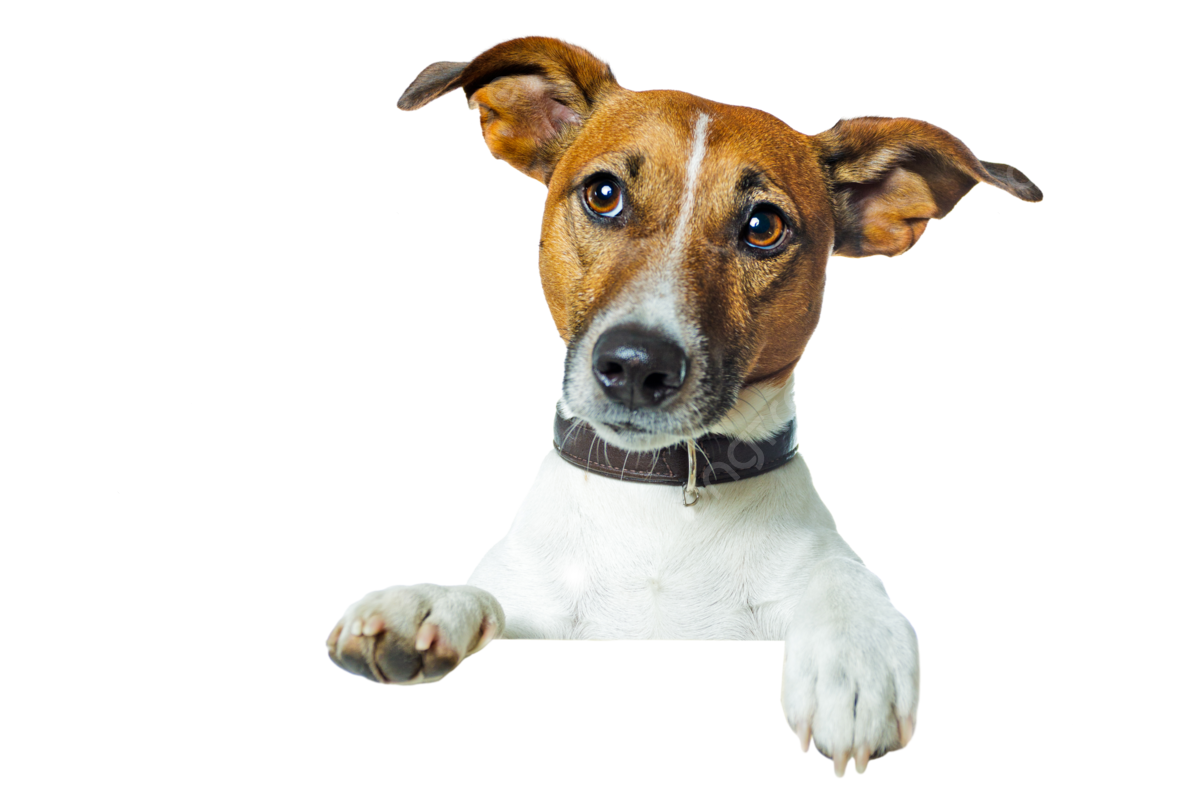
\includegraphics[width=0.45\linewidth]{Chapter1/Media/PLACEHOLDER.png}
    \caption{Diagram of 1D Rod Case, including original boundary conditions proposed for that case~\cite{}.}
    \label{fig1DRod}
\end{figure}


\subsubsection{Model Implementation}
The model implementation was designed to work using a configuration file that includes all the relevant parameters required to define a simulation. This ensures that the model will be robust enough to handle a wide range of simulations without needing any modifications. A summary of all the different parameters included in the file is shown in Table~\ref{tabDiffConfig1D}. A detailed explanation of each one of the groups and their relevant information is shown below. \textbf{Physical} includes the initial temperature and a list of the available materials and their thermophysical properties. \textbf{Geometrical} includes the geometric parameters; the model can only support rectangular shapes in this implementation and changes will be made when more complex geometries are studied. Sections must be defined with a material, the number of nodes for that specific section $N_s$, beginning and ending coordinates $x_0$ and $x_1$, and internal heat generation $q_V$. \textbf{Numerical} includes the numerical parameters; the model currently has both the Gauss-Seidel (GS) and Conjugate Gradient (CG) solvers implemented and both will be compared as a first step before performing the relevant studies discussed ahead. \textbf{Mesh} includes the option to choose from four different algorithms, as well as all relevant parameters for each of these alternatives. \textbf{Boundary Conditions} includes an array describing the boundaries for the model and can currently support Dirichlet, Neumann, and Convection boundary conditions. In addition, it supports variable temperatures for Dirichlet boundary conditions.

\begin{table}[ht]
	\centering
	\begin{tabular}{|l|c|p{0.5\linewidth}|}
		\hline
		Group & Parameter & Description \\
		\hline
		\multirow{3}{*}{Physical Data} & T0 & Initial value for temperature map. \\
					       & \multirow{2}{*}{materials} & List of vectors with thermophysical properties corresponding to each material. \\
		\hline
		\multirow{5}{*}{Geometrical Data} & width & Geometric dimension. \\
					          & height & Geometric dimension. \\
                              & \multirow{3}{*}{sections} & List of vectors indicating the distribution of materials in the simulation. Also includes amount of nodes and internal heat generation. \\
		\hline
		\multirow{7}{*}{Numerical Data} & scheme & Scheme for simulation. \\
					     & solver & Solver algorithm for simulation. \\
					     & maxIterations & Limit of iterations per timestep. \\
					     & endTime & Last instant of the simulation. \\
					     & timeStep & Time increment after each instant. \\
					     & tolNumeric & Tolerance for numerical solver. \\
					     & tolTemporal & Tolerance for steady-state convergence. \\
		\hline
		\multirow{5}{*}{Mesh Data} & meshAlgorithm & Algorithm for mesh generation. \\
					   & strength & Cubic algebraic mesh parameter. \\
					   & centering & Cubic algebraic mesh parameter. \\
					   & kappa & Power law mesh parameter. \\
					   & delta & Hyperbolic tangent mesh parameter. \\
		\hline
		\multirow{2}{*}{Boundary Data} & \multirow{2}{*}{boundaries} & List of vectors describing the boundary conditions on each side. \\
		\hline
	\end{tabular}
	\caption{Configuration file structure for 1D Rod Case. Showing the design structure for the metadata used to define the simulations.}
	\label{tabDiffConfig1D}
\end{table}


\subsubsection{Temporal Scheme}
One of the first numerical parameters to be evaluated in this project is the temporal scheme. This parameter determines the relevance that each time-step will have in the calculation of the next one. The \textbf{explicit} scheme, relies exclusively on information available from the current time-step, described as a function $f(T^{n-1})$ and requires a small enough time-step to ensure stability, given by Eq.~\eqref{eqDifftExplicit1D}. On the other hand, the \textbf{implicit} scheme relies exclusively on information from the time-step being currently calculated, being a function of $f(T^n)$. Finally, the \textbf{Crank-Nicolson} scheme employs a second-order scheme that averages the estimation made by both the explicit and implicit temporal schemes, being a function of $f(0.5 (T^{n-1} + T^n))$. 

\begin{equation}~\label{eqDifftExplicit1D}
    \Delta t_{max} = \frac{\Delta x^2}{2 \alpha}
\end{equation}


\subsubsection{Solver Comparison}
An additional decision to make when solving this kind of problems is the numerical solver to be used during simulations. While the matrix definition remains constant in both cases, as both require a sparse matrix in the form $A \mathbf{T} = b$, selecting the right solver can have a big impact in the performance of the solver. In this project, an initial comparison between the Gauss-Seidel (GS) and Conjugate Gradient (CG) algorithms will be made with the objective of evaluating performance and efficiency. A brief introduction to both algorithms is shown below before showing the results of said comparison.


\paragraph{Gauss-Seidel}
The GS method solves linear systems by iteratively cycling through each node in sequence and updating them by using the most recent values from its adjacent nodes. Each cell needs to be calculated directly by using Eq.~\eqref{eqSolverGS}, which delays the propagation of information from one cell to the others. While convergence is a guarantee when the matrix is diagonally dominant, it is susceptible to mesh size as it will directly impact the number of operations.

\begin{equation}~\label{eqSolverGS}
    T^{n+1}_P = \frac{1}{a_P} \left( b_P - \sum_{k \neq P} a_k T^*_{k} \right)
\end{equation}

\begin{algorithm}[ht]
\caption{Gauss-Seidel iterative solver}
\label{algGS}
\begin{algorithmic}[1]
    \Require Coefficient matrix $A$, RHS vector $\mathbf{b}$, initial guess $\mathbf{T}^0$, tolerance $\varepsilon$, maximum iterations $k_{\max}$
    \Ensure Solution vector $\mathbf{T}$
    \State $\mathbf{T} \gets \mathbf{T}^0$
    \For{$k = 1$ \textbf{to} $k_{\max}$}
        \For{$i = 1$ \textbf{to} $N$}
            \State $T_i \gets \dfrac{1}{a_{ii}} \!\left( b_i - \displaystyle\sum_{j \neq i} a_{ij}\, T_j \right)$
        \EndFor
        \If{$\|\mathbf{b} - A\mathbf{T}\| < \varepsilon$}
            \State \textbf{break}
        \EndIf
    \EndFor
    \Return $\mathbf{T}$
\end{algorithmic}
\end{algorithm}


\paragraph{Conjugate Gradient}
The CG method is an iterative Krylov subspace solver designed specifically for Symmetric Positive Definite (SPD) systems. For heat conduction problems, this matches the diffusion coefficient matrix since the interaction between two adjacent nodes is identical in both directions (symmetrical) and is diagonally dominant due to the accumulation term in $a_P$ (positive definite). Contrary to the GS method, rather than updating the values one by one, CG minimizes the residual over the sequence of search directions $\mathbf{p}_k$ that are mutually $A$-conjugate:

\begin{equation}~\label{eqSolverCG}
    \mathbf{p}^T_i A \mathbf{p}_j = 0, \qquad i \neq j
\end{equation}

This guarantees that no iteration undoes the progress made by previous ones. Because of this capacity of propagating information, CG converges in maximum $N$ iterations, being $N$ the amount of unknowns. It is also important to highlight that CG is only valid for SPD systems. As it will be explained in Chapter~\ref{chapConvection}, once symmetry is broken due to the convective term, the solver algorithm needs to be changed to a more generalized variant to be able to handle non-SPD scenarios.

\begin{algorithm}[ht]
\caption{Conjugate Gradient solver}
\label{algCG}
\begin{algorithmic}[1]
    \Require SPD coefficient matrix $A$, RHS vector $\mathbf{b}$, initial guess $\mathbf{T}^0$, tolerance $\varepsilon$, maximum iterations $k_{\max}$
    \Ensure Solution vector $\mathbf{T}$
    \State $\mathbf{r}^0 \gets \mathbf{b} - A\mathbf{T}^0$;\quad $\mathbf{p}^0 \gets \mathbf{r}^0$;\quad $\mathbf{T} \gets \mathbf{T}^0$
    \For{$k = 0, 1, 2, \ldots, k_{\max}$}
        \State $\alpha_k \gets \dfrac{\mathbf{r}^k \cdot \mathbf{r}^k}{\mathbf{p}^k \cdot A\,\mathbf{p}^k}$
        \State $\mathbf{T}^{k+1} \gets \mathbf{T}^k + \alpha_k\,\mathbf{p}^k$
        \State $\mathbf{r}^{k+1} \gets \mathbf{r}^k - \alpha_k\, A\,\mathbf{p}^k$
        \If{$\|\mathbf{r}^{k+1}\| < \varepsilon$}
            \State \textbf{break}
        \EndIf
        \State $\beta_k \gets \dfrac{\mathbf{r}^{k+1} \cdot \mathbf{r}^{k+1}}{\mathbf{r}^k \cdot \mathbf{r}^k}$
        \State $\mathbf{p}^{k+1} \gets \mathbf{r}^{k+1} + \beta_k\,\mathbf{p}^k$
    \EndFor
    \Return $\mathbf{T}^{k+1}$
\end{algorithmic}
\end{algorithm}


\paragraph{Results}
Solver performance is evaluated using two metrics: the number of inner iterations required to reach convergence at each time-step, and the final residual $\|\mathbf{b} - A\mathbf{T}\|$ after convergence. The comparison is carried out on the \textbf{1D Rod Case}~\cite{} extended with an internal heat source $q_V$, which introduces a parabolic steady-state profile that can be directly compared against the analytical solution given by Eq.~\eqref{eq1DAnalyticalSol}. Both solvers use $N = 100$ nodes, $\Delta t = 0.5\,\text{s}$, a Crank-Nicolson temporal scheme, and a uniform mesh. The results are shown in Figure~\ref{figDiffCompSolver}.

CG outperforms GS by a considerable margin on both metrics. This is consistent with the structural properties described above: the diffusion matrix is SPD, so CG propagates information globally through its $A$-conjugate search directions and is guaranteed to converge in at most $N$ steps. GS updates nodes one at a time, propagating information only one cell per iteration, and therefore requires many more sweeps to resolve long-range temperature gradients. Based on these results, CG was selected as the solver for all subsequent numerical studies in this chapter.

\begin{figure}[ht]
    \begin{tabular}{cc}
        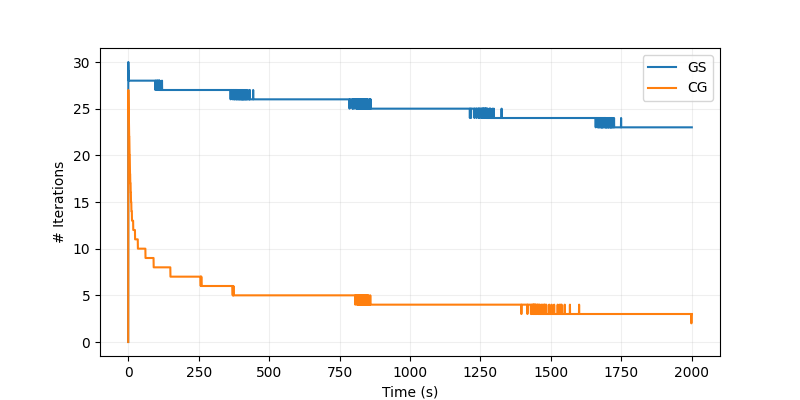
\includegraphics[width=0.45\linewidth]{Chapter1/Media/SolverComparisonIterations.png} & 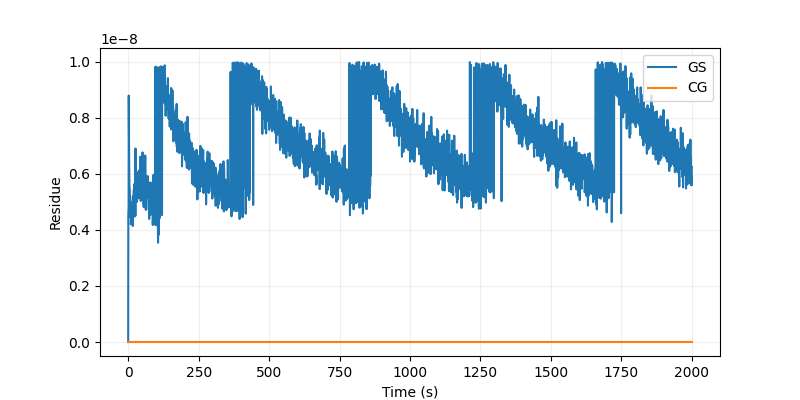
\includegraphics[width=0.45\linewidth]{Chapter1/Media/SolverComparisonResidue.png} \\
        \textit{Iterations} & \textit{Residue} \\
    \end{tabular}
    \caption{\textit{Performance comparison between Gauss-Seidel and Conjugate Gradient solvers. Number of iterations until solution (left) and solver residual after convergence (right).}}
    \label{figDiffCompSolver}
\end{figure}


\subsubsection{Numerical Parameters Study}
For this test, the time step $\Delta t$ and the number of nodes $N$ are modified to analyze the number of iterations and compare them with the analytical solution. Both parameters will be independently swept across their respective range of values, while keeping the other parameter at a constant value. A summary of the values for each one of these parameters is shown in Table \ref{tabDiffNumerical1D}, highlighting the values used for the base case.

\begin{table}[ht]
    \centering
    \begin{tabular}{|c|c|}
        \hline
        Parameter & Values \\
        \hline
        $\Delta t$ & 0.1, \textbf{0.5}, 1.0, 2.0, 5.0 \\
        $N$ & 50, \textbf{100}, 200, 400 \\
        \hline
    \end{tabular}
    \caption{\textit{Detail of numerical parameters to be studied. Each variable will remain at their respective highlighted value while the other one sweeps through their range.}}
    \label{tabDiffNumerical1D}
\end{table}


\paragraph{$\Delta t$ Sweep}
The results obtained from the tests explained above are shown in Figure \ref{figDiffResults1DA}. As expected, the number of iterations remains unchanged for the explicit scheme, as it is meant to be a direct calculation. On the other hand, both the Crank-Nicolson and implicit schemes require more iterations per time step as it increases. This is mainly due to the accumulation term decreasing in magnitude as $\Delta t$ increases, while the adjacent node coefficients do not decrease with $\Delta t$. This in turn makes the system less diagonally dominant and slower to converge. Compared to the analytical solution, the explicit scheme shows a significant error for $0.1 < \Delta t$, while a small increase could be seen for the Crank-Nicolson and implicit schemes. As a second-order accurate method, Crank-Nicolson shows lower error compared to implicit, which is a first-order accurate method. Overall, the Crank-Nicolson scheme has shown better performance in terms of number of iterations needed and precision compared to the analytical solution. Furthermore, the results for explicit seem to stagnate at a constant value after the lowest time step value tested, suggesting that the limit set by Eq. \ref{eqDifftExplicit1D} has been exceeded. The computation time is seen to be similar between the Crank-Nicolson and implicit schemes, with a small advantage for the implicit scheme.

\begin{figure}[ht]
    \begin{tabular}{cc}
        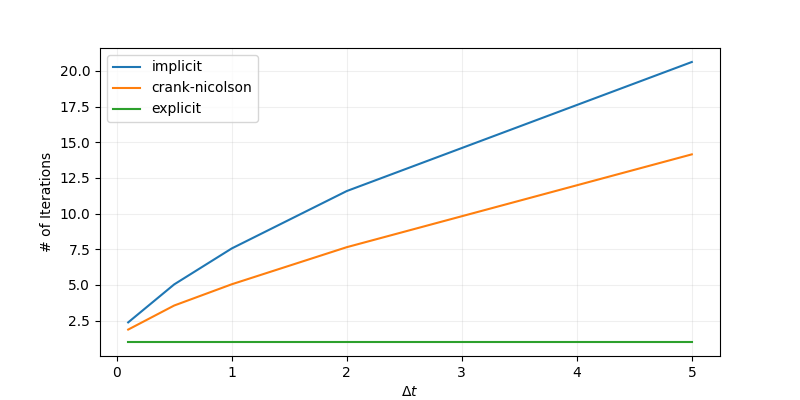
\includegraphics[width=0.45\linewidth]{Chapter1/Media/tSweepIterations.png} & 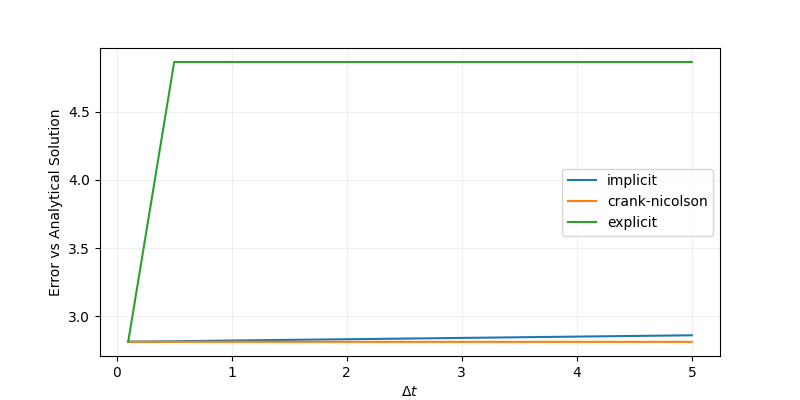
\includegraphics[width=0.45\linewidth]{Chapter1/Media/tSweepAnalytical.png} \\
        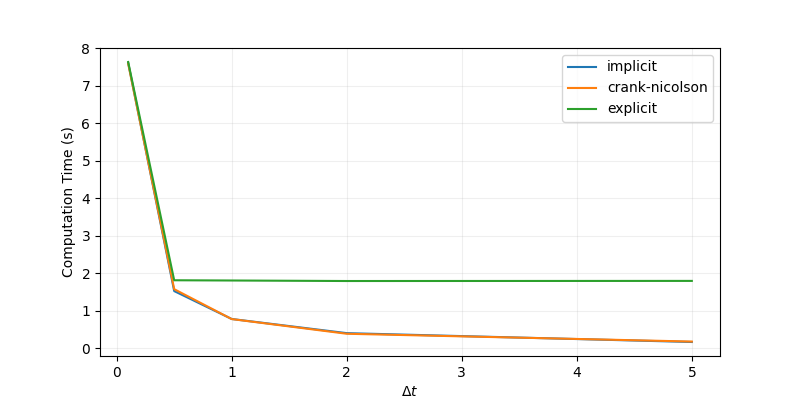
\includegraphics[width=0.45\linewidth]{Chapter1/Media/tSweepTime.png} & 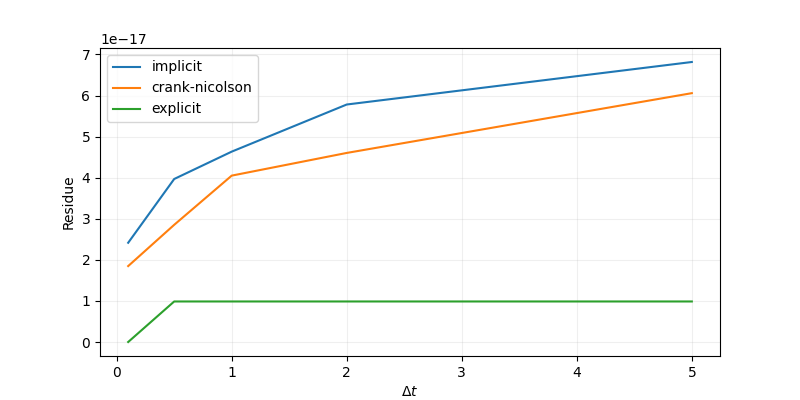
\includegraphics[width=0.45\linewidth]{Chapter1/Media/tSweepResidue.png} \\
    \end{tabular}
    \caption{\textit{$\Delta t$ sweep results.}}
    \label{figDiffResults1DA}
\end{figure}


\paragraph{$N$ Sweep}
The results obtained for the tests explained above are shown in Figure \ref{figDiffResults1DB}. Similarly to the previous case, the explicit scheme is a direct calculation and does not require more iterations. In addition, both the Crank-Nicolson and implicit schemes show an increase in the number of iterations as the mesh is refined, with Crank-Nicolson showing better performance overall. Since a larger mesh means more finite volumes, the amount of calculations performed by the model will increase. Compared to the analytical solution, the explicit scheme still showed higher values when compared to the Crank-Nicolson and implicit schemes; however, it seems to get closer as the number of nodes increases. In terms of computation time, both the Crank-Nicolson and implicit schemes saw a slight increase, while the explicit scheme saw a major difference as the mesh got finer.

\begin{figure}[ht]
    \begin{tabular}{cc}
        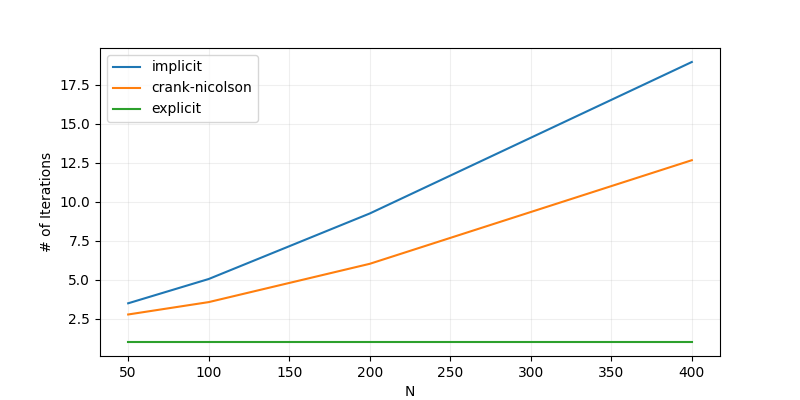
\includegraphics[width=0.45\linewidth]{Chapter1/Media/NSweepIterations.png} & 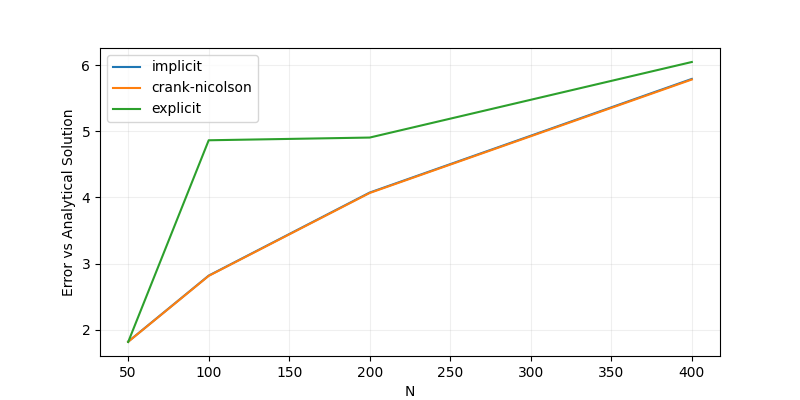
\includegraphics[width=0.45\linewidth]{Chapter1/Media/NSweepAnalytical.png} \\
        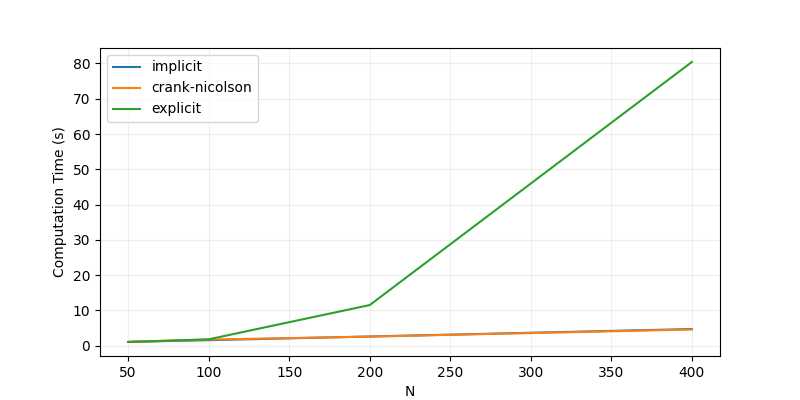
\includegraphics[width=0.45\linewidth]{Chapter1/Media/NSweepTime.png} & 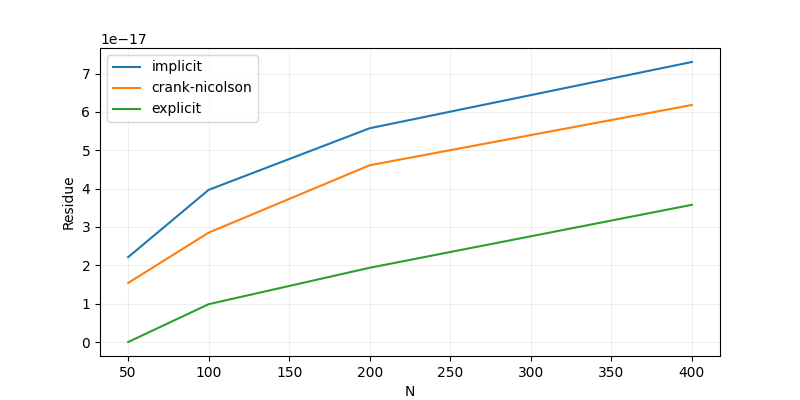
\includegraphics[width=0.45\linewidth]{Chapter1/Media/NSweepResidue.png} \\
    \end{tabular}
    \caption{\textit{$N$ sweep results.}}
    \label{figDiffResults1DB}
\end{figure}


\subsubsection{Model Validation}
In addition to the Dirichlet boundary condition established in the problem statement, Neumann and Convection boundary conditions have also been implemented in the model. Furthermore, support for variable temperatures for Dirichlet boundary conditions was implemented. To validate this implementation, a comparison will be made with the analytical solution for a steady-state scenario with the transient-state model once it reaches equilibrium.

At steady state the time derivative vanishes and the 1D governing equation reduces to:

\begin{equation}~\label{eq1DAnalytical}
    \frac{d}{dx}\!\left(\lambda \frac{dT}{dx}\right) + q_V = 0
\end{equation}

For uniform $\lambda$ and $q_V = 0$, this integrates to a linear temperature profile $T(x) = A + Bx$, with constants $A$ and $B$ determined by the two boundary conditions. Table~\ref{tabDiff1DAnalytical} summarises the closed-form solutions for each of the five boundary-condition pairs tested. For Cases 2 and 4 (Robin), the temperature at the convective wall $T^*$ follows from the continuity of heat flux between the fluid and the solid at steady state.

\begin{table}[ht]
    \centering
    \renewcommand{\arraystretch}{2.2}
    \begin{tabular}{|c|l|l|}
        \hline
        Case & Boundary Conditions & Analytical Solution $T(x)$ \\
        \hline
        1 & Neumann (W) -- Dirichlet (E)
          & $T_E + \dfrac{\dot{q}_W}{\lambda}(L - x)$ \\
        2 & Robin (W) -- Dirichlet (E)
          & $T_w^* + (T_E - T_w^*)\dfrac{x}{L}$,\quad $T_w^* = \dfrac{hL\,T_\infty + \lambda\,T_E}{hL + \lambda}$ \\
        3 & Dirichlet (W) -- Neumann (E)
          & $T_W + \dfrac{\dot{q}_E}{\lambda}\,x$ \\
        4 & Dirichlet (W) -- Robin (E)
          & $T_W + (T_e^* - T_W)\dfrac{x}{L}$,\quad $T_e^* = \dfrac{\lambda\,T_W + hL\,T_\infty}{\lambda + hL}$ \\
        5 & Variable Dirichlet (W) -- Dirichlet (E)
          & $T_W(t) + \bigl(T_E - T_W(t)\bigr)\dfrac{x}{L}$,\quad $T_W(t) = 100 + 50\cos\!\!\left(\dfrac{0.01\,t}{5\pi}\right)$ \\
        \hline
    \end{tabular}
    \caption{Analytical steady-state solutions for each boundary-condition pair. $\dot{q}_W$ and $\dot{q}_E$ denote the prescribed heat flux entering the domain at the west and east faces respectively; $h$ is the convective heat transfer coefficient and $T_\infty$ the far-field fluid temperature.}
    \label{tabDiff1DAnalytical}
\end{table}

A summary of the pairs of boundary conditions used for the tests is shown in Table~\ref{tabDiff1DBoundaryCases}, while comparisons with the steady-state solution are shown in Figure~\ref{figDiff1DAnalSol}. An additional case is included to test the proper implementation of the variable temperature Dirichlet boundary condition. As shown, all pairs evaluated accurately matched the analytical solution. Furthermore, the configuration file can now provide mathematical expressions instead of constant values when defining Dirichlet boundary conditions, as shown by the temperature profile in Case 5. This capability can now easily be scaled up towards other functions in the model.

\begin{table}[ht]
    \centering
    \begin{tabular}{|c|c|}
        \hline
        Case & Boundary Conditions \\
        \hline
        1 & Neumann-Dirichlet \\
        2 & Convection-Dirichlet \\
        3 & Dirichlet-Neumann \\
        4 & Dirichlet - Convection \\
        5 & $T_{(t)} = 100 + 50 \cos \left( \frac{0.01 t}{5 \pi} \right)$ \\
        \hline
    \end{tabular}
    \caption{\textit{Cases for model validation. Each case describes a Left-Right pair of boundary conditions to be tested with the 1D Rod Case.}}
    \label{tabDiff1DBoundaryCases}
\end{table}

\begin{figure}[ht]
    \begin{tabular}{cc}
        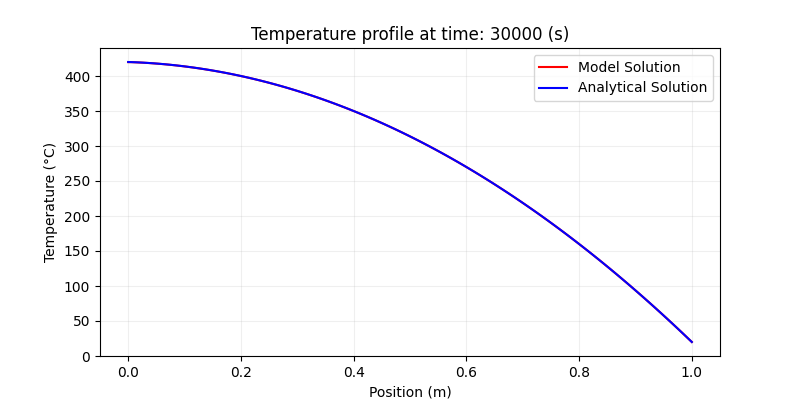
\includegraphics[width=0.45\linewidth]{Chapter1/Media/BoundaryND.png} & 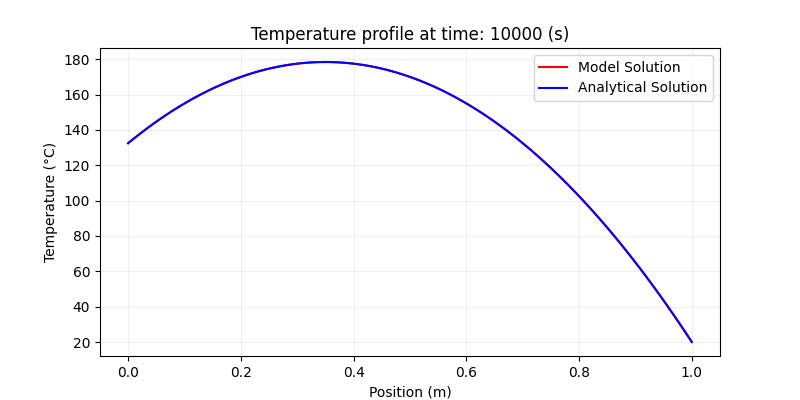
\includegraphics[width=0.45\linewidth]{Chapter1/Media/BoundaryCD.png} \\
	\scriptsize{\textit{Case 1}} & \scriptsize{\textit{Case 2}} \\
        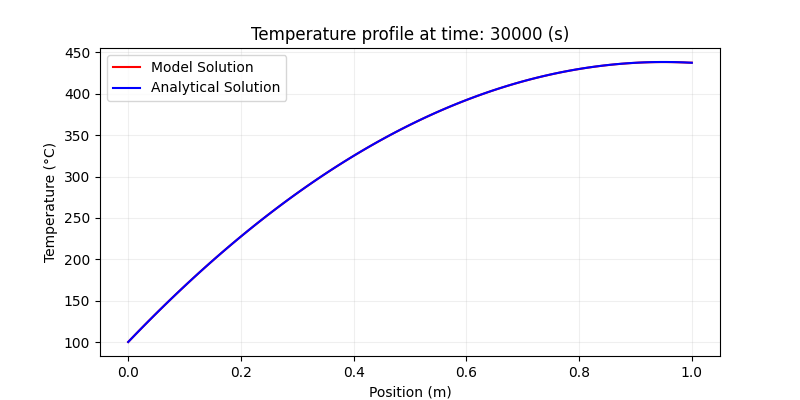
\includegraphics[width=0.45\linewidth]{Chapter1/Media/BoundaryDN.png} & 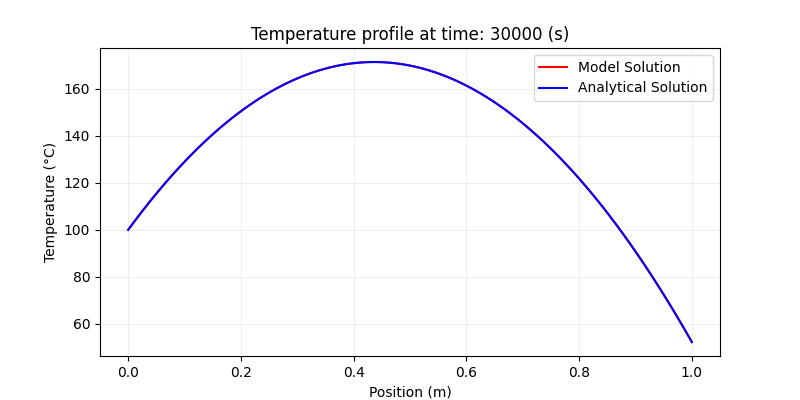
\includegraphics[width=0.45\linewidth]{Chapter1/Media/BoundaryDC.png} \\
	\scriptsize{\textit{Case 3}} & \scriptsize{\textit{Case 4}} \\
        \multicolumn{2}{c}{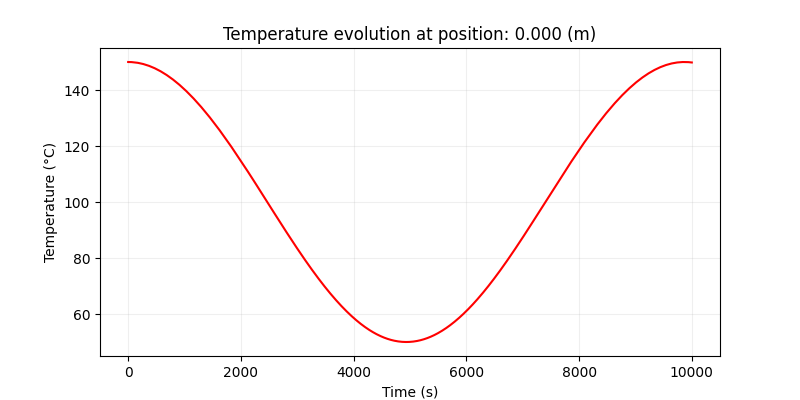
\includegraphics[width=0.45\linewidth]{Chapter1/Media/BoundaryVD.png}} \\
	\multicolumn{2}{c}{\scriptsize{\textit{Case 5}}} \\
    \end{tabular}
    \caption{\textit{Comparison of model results with analytical solutions and implementation of mathematical expression reading for Dirichlet boundary condition.}}
    \label{figDiff1DAnalSol}
\end{figure}

